\documentclass[a4paper]{ctexart}    %ctexart
\usepackage[margin=1cm]{geometry}
\usepackage{amsmath, mathrsfs, amsfonts}
\usepackage{amssymb}
\usepackage[utf8]{inputenc}
\usepackage{pgfplots}
\usepackage{xcolor}
\usepackage{minted}
\usepackage{tikz}
\usepackage{tkz-euclide}





\begin{document}
\begin{minted}[mathescape,
               linenos,
               numbersep=5pt,
               gobble=0,
               frame=lines,
               framesep=2mm]{tex}
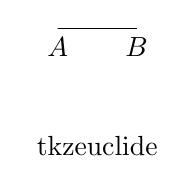
\begin{tikzpicture}
    \begin{scope}[xshift=6cm]
        \node at (.5,-1.5){tkzeuclide};
    \tkzDefPoints{0/0/A,1/0/B}     % 定义多个点
    \tkzDrawSegments(A,B)          % 绘制线段
    \tkzLabelPoints[below](A,B)    % 绘制标签
    \end{scope}
\end{tikzpicture}
\end{minted}

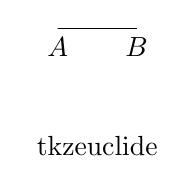
\begin{tikzpicture}
    \begin{scope}[xshift=6cm]
        \node at (.5,-1.5){tkzeuclide};
    \tkzDefPoints{0/0/A,1/0/B}     % 定义多个点
    \tkzDrawSegments(A,B)          % 绘制线段
    \tkzLabelPoints[below](A,B)    % 绘制标签
    \end{scope}
\end{tikzpicture}


\end{document}
